\chapter{Architecture and Implementation}
\label{ch:architecture-and-implementation}

\section{Architecture of the Software}

  \subsection{Adaptation Loop}


  The SAA adaptation approach is defined as a loop, that cyclically updates every component contained in the loop.
  The adaptation loop is shown in figure \ref{fig:adaptation-loop} and consists of the Big Data pipeline and the \emph{resources} contain all registered and monitored to the \emph{Monitoring and Analysis} component. 
  Both the Big Data pipeline and the resources send the gathered monitoring information at a time step $P_t$ or $S_t$ respectively to the \emph{Monitoring and Analysis} component, where $t$ denotes the current time step.

  The Monitoring and Analysis component then uses the monitoring data $P_t$ and $S_t$, and calculates an action $A_{t+1}$ as an update for the resources, where $t+1$ denotes the next time step.
  
  This received action $A_{t+1}$ is then used by the Resource components to reconfigure the resources if necessary.
  The adaptation uses monitoring of tasks and resources to retrieve the monitoring data $P_t$, $S_t$.
  
  Monitoring component is necessary to obtain information about failures or performance fluctuations along with under-, over-utilization of resources.
  The monitoring data, therefore, provides feedback if a resource is able to handle additional load, and thus, more tasks will potentially be mapped to it for execution. 
  In case that the resource is not capable of handling the current load, less demanding tasks will be mapped to that resource in future scheduling cycles and it will be reconfigured accordingly.

  A monitored resource information consists of the CPU, memory and storage utilization, in addition to network bandwidth usage.
  The Big Data pipeline and resources send their monitoring data $P_t$, $S_t$ respectively to the Monitoring and Analysis component.
  Afterward, given those monitoring data, the analyzer will determine the next action $A_{t+1}$ of the resources.
  The monitoring feedback will be periodically retrieved from all registered resources and provided to the analyzer.
  In case of a resource side failure, the monitoring mechanism will be alerted of the occurred anomaly.  
  The analyzer uses this monitoring data to decide if any actions $a \in A$ on the current scheduling plan have to be applied.
  
  \begin{figure}[h!]
    \centering
     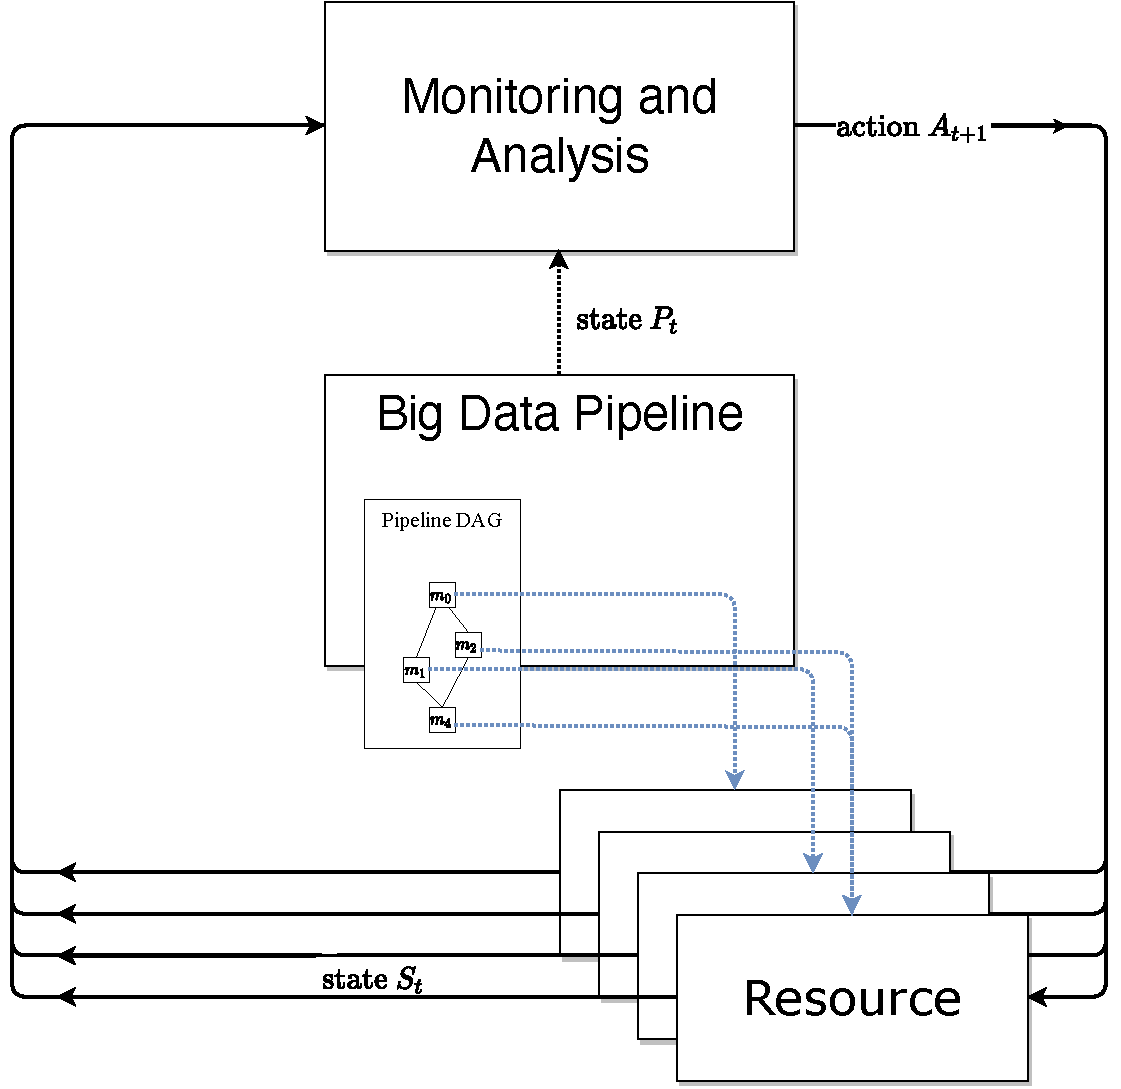
\includegraphics[width=\columnwidth]{figures/monitoring_with_inner_resources.drawio.pdf}
    \caption{Adaptation Loop}
    \label{fig:adaptation-loop}
\end{figure}
The following actions $A$ are considered in the adaptation approach:

\paragraph*{Resource load within expected parameters $(S_1)$} 
When tasks on resources are well mapped and no action has to be taken for these resources, this is denoted in the action set $A_{t+1}$ as the state $S_1$. This state is achieved when a resource is running within expected parameters, the estimated time of completing a task is not exceeded or other anomalies occur.

\paragraph*{Resource load under expected parameters $(S_2)$} 
When the monitoring component detects under-utilization of a resource, tasks of the pipeline are mapped to it to be efficiently utilized. This state is categorized as $S_2$ in the analyser and the action set will be modified to improve the utilization of resources grouped into $S_2$. 

\paragraph*{Resource load over expected parameters $(S_3)$} 
If a resource is over-utilized, there are multiple options. If it is detected that horizontal scaling solves the over-utilization and the resource instance is capable of being scaled up, it will be reconfigured to be within expected utilization levels. Furthermore, if an ill-defined task is detected and was mapped to a resource that isn't capable to fulfill the computation within a reasonable time frame, this task will be migrated to another resource. 
This is categorized as $S_3$ in the analyser, and the action set will be modified, so that resources grouped in $S_3$ will be less utilized with the upcoming updates of the action set. \cite{kimovskiBigDataPipeline2022}


\section{Monitoring}

\section{Data Preprocessing and Analysis}

  \subsection{Alibaba Resource Analysis}
  \subsection{LSTM Architecture}
  \label{sec:lstm-architecture-and-implementation}

    The LSTM model was implemented with \nameref{sec:pytorch-evaluation-setup}, an open-source machine learning library for Python.
    \begin{figure}
      \centering
      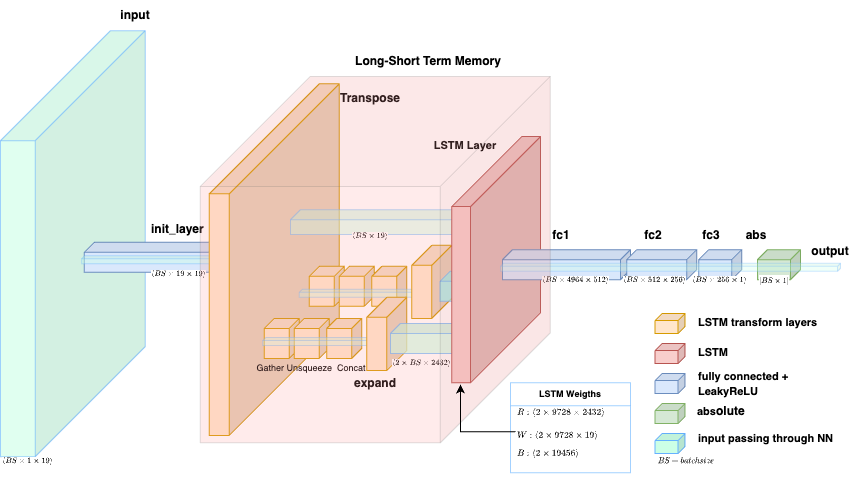
\includegraphics[scale=0.5]{figures/current_lstm_model.png}
      \caption{LSTM Model Architecture}
      \label{fig:lstm-model-architecture}
    \end{figure}
    As can be seen in figure \ref{fig:lstm-model-architecture} the input vector consisting of a pipeline task batch is forwarded to the \emph{initial layer}. This initial layer then creates an internal state and the initial hidden state depending on the size of the input (the data points in a time series forecasting data batch).
    The general LSTM prediction model is split into two smaller LSTM components that each predict the utilisation of one resource unit. A resource unit is either the CPU usage or the allocated memory. At creation these LSTM components use the length of the input as the expected input size and quality of the prediction performance heavily depends on the chosen hidden layer size as well as the number of \nameref{sec:stacked-lstm} layers.
    The final LSTM output of either resource unit is then send to traditional sequential layers that use batch normalisation as the generalisation strategy.
    % TODO describe batch normalization
    Afterwards, the output of those sequential layers is concatenated column-wise as a label vector of the form $\left[(cpu_1, mem_1), \dots, (cpu_{bs}, mem_{bs})\right]$ where $bs$ denotes the batch size or number of data points in the batch.

    % TODO Explain ReLU and other layers



  % \lstinputlisting[
  %   language=Python, 
  %   caption=LSTM Architecture, 
  %   label=lst:pmse-python-class,
  %   captionpos=b,
  %   keywordstyle=\color{blue},
  %   frame=single,
  %   morekeywords={torch, nn, Module, Tensor, self},
  %   backgroundcolor=\color{gray!10!white},
  %   breaklines=true,
  %   numberstyle=\tiny\color{black},
  %   numbers=left,
  %   ]{code_samples/lstm_architecture.py}

  

\section{Adaptation}
  \subsection{Resource Prediction}
  % flow chart of resource prediction
  \subsection{DataFrame Scaler}
  \subsection{Penalty Mean Squared Error Loss Function}
  \label{sec:penalty-mse-loss-function-architecture-and-implementation}

    The \emph{Penalty Mean Squared Error (PMSE) loss function} is a custom loss function based on the commonly used \emph{Mean Squared Error (MSE) loss function} \cite{koksoyMultiresponseRobustDesign2006} for regression. Penalty in this loss function refers to increasing the loss of predicted values $\hat{y}_i$ that are lower than the actual value $y_i$.
    $$MSE = \frac{1}{N} \sum_{i = 1}^{N}\left(y_i - \hat{y}_i\right)^2$$

    $$Penalty = [0, \infty]$$
    $$\hat{y'}_i = 
    \begin{cases}
      \hat{y}_i,  & \hat{y}_i >= y_i \\
      \hat{y}_i - Penalty, & \hat{y}_i < y_i
    \end{cases}$$

    $$PMSE = \frac{1}{N} \sum_{i = 1}^{N}\left(y_i - \hat{y'}_i\right)^2$$

    
    The \texttt{PenaltyMSELoss} class inherits from the PyTorch Module package in order to be able to use it as the loss function for the error calculation of the predicted and actual values.
    The \texttt{PenaltyMSELoss} class constructor has two parameters, the \texttt{self} keyword that is used to access instance parameters, and the \texttt{penalty} parameter, that is expected to be of type \texttt{float}.
    Inside the class constructor, a \texttt{MSELoss} instance will be created in order to calculate the final loss values based on the mean square error calculation.
    

    \lstinputlisting[
      language=Python, 
      caption=Penalty Mean Squared Error Python Class, 
      label=lst:pmse-python-class,
      captionpos=b,
      keywordstyle=\color{blue},
      frame=single,
      morekeywords={torch, nn, Module, Tensor, self},
      backgroundcolor=\color{gray!10!white},
      ]{code_samples/pmse.py}


